% %% %%%%%%%%%%%%%%%%%%%%%%%%%%%%%%%%%%%%%%%%%%%%%%%%%%%%%%%%%%
% intro-bridge.tex
%
% Author:  Mauricio Matamoros
% License: MIT
%
% %% %%%%%%%%%%%%%%%%%%%%%%%%%%%%%%%%%%%%%%%%%%%%%%%%%%%%%%%%%%
%!TEX root = ../practica.tex
%!TEX root = ../references.bib

% CHKTEX-FILE 1
% CHKTEX-FILE 13
% CHKTEX-FILE 46

\subsection{El puente rectificador}%
\label{seq:intro-bridge}

\begin{wrapfigure}{r}{0.3\columnwidth}
	\centering
	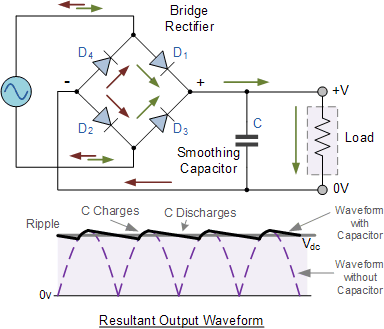
\includegraphics[width=0.3\columnwidth]{img/bridge.png}
	\caption[Rectificador de onda completa]{Rectificador de onda completa\footnotemark{}}%
	\label{fig:bridge}
\end{wrapfigure}
\footnotetext{Fuente de imagen: \url{https://lasopaeden528.weebly.com/bridge-rectifier-calculator.html}}
Un puente rectificador o rectificador de onda completa es un arreglo de 4 diodos que permiten el paso de la corriente en un sólo sentido, invirtiendo así la parte negativa de una señal de AC respecto a su voltaje de referencia.
Los puentes rectificadores son un componente fundamental en los transformadores de corriente de AC a DC.

El circuito funciona de la siguiente manera.
En la primera parte del ciclo, cuando el voltaje comienza a aumentar, la corriente fluye de la parte norte del puente (arriba) a través de $D_1$ hacia la carga, y luego de regreso por $D_2$ hacia el neutro (véase~\Cref{fig:bridge}).
En esta primera etapa, $D_3$ y $D_4$ actuan como barreras evitando que la corriente fluya directamente de la fase al neutro (corto circuito).
Tras pasar por la carga, el voltaje en en el ánodo de $D_4$ ha caído y es menor que en el cátodo, por lo que no habrá flujo de corriente en esta dirección, pero aún es positivo respecto al neutro ($V_{N}=0$), por lo que la corriente tendrpa que pasar por $D_1$.
De forma análoga, el voltaje en el cátodo de $D_3$ es menor que en el ánodo, por lo que tampoco habrá flujo en esta dirección.

En la segunda parte del ciclo, el voltaje de fase disminuye respecto al neutro, por lo que la corriente fluye de la parte sur del puente (abajo) a través de $D_3$ hacia la carga, y luego de regreso por $D_4$ hacia la fase (véase~\Cref{fig:bridge}).
En esta segunda etapa, $D_1$ y $D_2$ actuan como barreras evitando que la corriente fluya directamente del neutro a la fase (corto circuito).
Tras pasar por la carga, el voltaje en en el ánodo de $D_2$ ha caído y es menor que en el cátodo, por lo que no habrá flujo de corriente en esta dirección, pero aún es positivo respecto a la fase ($V_{N}=0$), por lo que la corriente tendrpa que pasar por $D_4$.
De forma análoga, el voltaje en el cátodo de $D_1$ es menor que en el ánodo, por lo que tampoco habrá flujo en esta dirección.
